\documentclass[11pt,a4paper]{article}
\usepackage{parskip}
\usepackage[top=1in, left=1in, right=1in, bottom=1in]{geometry}
\usepackage{amsmath}
\usepackage{graphicx}
\usepackage{titling}

\title{Examples of Reducing Training Time\\ with More Data}
\author{Michael Wu, Brando Miranda, He Sun}

\begin{document}
\maketitle

\section{Overview}

	In most machine learning problems, we tend to think that training algorithms require more computation time as the number of training samples increases. In this paper we discuss two contexts in which this is not true. In the case of SVM optimization, assuming some desired generalization error, the PEGASOS algorithm statistically needs less runtime with more data. In the case of learning halfspaces over sparse vectors, more training examples reduce the training runtime from exponential to polynomial time.

%%%%%%%%%%%%%%%%%%%%%%%%%%%%%%%%%%%%%%%%%%%%%%%%%%%

\section{SVM Optimization}

\subsection{Introduction}

The traditional runtime analysis for machine learning models, such as SVM, involve minimizing optimization errors for regularized empirical loss function obtained from training data. This naturally leads to the conclusion that runtime increases as the training set size increases. However, our ultimate goal in machine learning is to study generalization error, of which optimization error is only one component. Hence, the traditional analysis does not provide information about runtime as a function of generalization error level. \\

In this section, we will analyze runtime for regularized SVM with linear kernel and claim that a subgradient-based algorithm PEGASOS can actually reduce runtime as the training set size increases. However, two other algorithms, Dual Decomposition and SVM-Perf are not exactly the same case. For them, runtime first decreases but then increases as the training set size increases. \\

In the following subsections, we will first introduce the regularized SVM with linear kernel as well as three algorithms, PEGASOS, SVM-Perf and Dual Decomposition. We will also discuss error decomposition for generalization error. Based on these knowledge, we will proceed to study extreme regimes: The Data Bounded Regime, which involves limited data but unlimited computational resources and The Data-Laden Regime, which involves unlimited data but limited computational resources. The analysis for these two cases serve as cornerstones for the following analysis of the Intermediate Regime.

\subsection{Regularized SVM with linear kernel setting}

The idea of SVM with linear kernel is to find a predictor $w\in R^d$ that predicts $y\in\{0,1\}$ with the largest margin based on a classifier $\mbox{sign}(<w,x>)$, where $x$ is a feature vector. Assuming our data $\{(x_i,y_i)\}_{i=1}^m$ are i.i.d. drawn from an underlying distribution $P(X,Y)$, the empirical loss with regularization for SVM with linear kernel can be written as:
\begin{equation}
\hat{f}_{\lambda}(w)=\hat{l}(w)+\frac{\lambda}{2}||w||^2
\end{equation}
where $\hat{l}(w)=\frac{1}{m}\sum_i l(w;(x_i,y_i))$ and $l(w;(x,y))=\mbox{max}\{0,1-y<w,x>\}$ is the hinge loss.

\subsection{Three algorithms for SVM}

\begin{enumerate}
\item \emph{Dual Decomposition}: Traditional algorithms for SVM treat the problem as a typical nonlinear optimization problem. They use interior point method and basically perform a Newton step for each iteration, which takes $O(m^3)$ time. However, Dual Decomposition algorithm makes use of the unique structure of SVM dual form. In particular, it only focuses on a subset of data points for each iteration, leading to $O(dm^2 \mbox{log}(\frac{1}{\epsilon_{acc}}))$ runtime, where $\epsilon_acc$ is the optimization error. Note that the complexity scales up with $m^2$
\item \emph{SVM-Perf}: This algorithm borrows ideas from cutting plane method and achieves runtime $O(\frac{md}{\lambda \epsilon})$. The complexity scales up with $m$.
\item \emph{PEGASOS}: This algorithm is built on traditional stochastic subgradient descent method, which achieves runtime $O(\frac{d}{\lambda\epsilon})$ with high probability. The complexity does not scale up with $m$.
\end{enumerate}

\subsection{Error Decomposition}

In this subsection, we decompose generalization error to approximation error, estimation error and optimization error. Before discussing about errors, we first introduce different predictors as follows:
\begin{enumerate}
\item $\bar{w}$: $\bar{w}$ is defined as the minimizer of SVM optimization using training data. Namely, $\bar{w}:=\mbox{argmin}_w \hat{f}_{\lambda}(w)$, where $\hat{f}$ represents the empirical loss function based on training data. 
\item $\tilde{w}$: $\tilde{w}$ is the predictor we actually obtained when solving $\mbox{argmin}_w \hat{f}_{\lambda}(w)$. Note that we cannot always achieve the precise minimizer for $\mbox{argmin}_w \hat{f}_{\lambda}(w)$ in practice, thus we can only rely on $\tilde{w}$.
\item $w^{*}$: $w^{*}:=\mbox{argmax}_w f_{\lambda}(w)$, where $f$ represents the true regularized loss function ($f_{\lambda}(w)=l(w)+\frac{\lambda}{2}||w||^2$). Namely, $w^{*}$ is the minimizer of the true SVM optimization.
\item $w_0$: Reference predictor, which is a minimizer of the true SVM optimization from a broader class of predictors.
\end{enumerate}
The generalization error for $\tilde{w}$, i.e. $l(\tilde{w})$, can be decomposed as follows:
\begin{equation}
l(\tilde{w})-l(w_0)=(l(\tilde{w})-l(\bar{w}))+(l(\bar{w})-l(w^{*}))+(l(w^{*})-l(w_0))
\end{equation}
The first term is the optimization error. The second is the estimation error, which is caused by minimizing the empirical loss instead of the true loss. The third is the approximation error, which is due to the fact that the space of predictors that we consider does not contain all possible predictors.

\subsection{Runtime analysis for Data Bounded Regime}

In this regime, we assume data is limited, whereas the computational power is unlimited. Therefore, we could ignore optimization error. It is reasonable to consider the training set size as a function of some desired generalization error level $\epsilon$. In particular, the sample complexity is $m=O(\frac{||w^{*}||^2}{\epsilon^2})$

\subsection{Runtime analysis for Data-Laden Regime}

In this regime, we assume another extreme case, where data is unlimited but computational power is limited. Our goal is to consider runtime as a function of a desired generalization error for each of three algorithms introduced before. The way to approach this is first decomposing generalization error, and an upper bound each part by a few of inequalities. With imposing generalization error level $\epsilon$, we could play algebra and produce bounds for parameter $\epsilon_{acc}$, the optimization error, $\lambda$, the regularization parameter and $m$, the training set size in terms of $\epsilon$. In the end, we plug in all these bounds into the runtime complexity expression for all three algorithms.\\
In details, the decomposition is
\begin{equation*}
l((\tilde{w})=l(w_0)+(f_{\lambda}(\tilde{w})-f_{\lambda}(w*))+(f_{\lambda}(w*)-f_{\lambda}(w_0))+\frac{\lambda}{2}||w_0||^2-\frac{\lambda}{2}||\tilde{w}||^2
\end{equation*}
We could bound each term of the RHS and obtain the following inequality:
\begin{equation}
l((\tilde{w}) \leq l(w_0)+2\epsilon_{acc}+\frac{\lambda}{2}||w_0||^2+0+O(\frac{1}{\lambda m})
\label{equ1}
\end{equation}
. For a specific generalization error $\epsilon$, we could bound the last three terms in the RHS above by $O(\epsilon)$. By some simple algebra, we have:
$\epsilon_{acc} \leq O(\epsilon)$, $\lambda \leq O(\frac{\epsilon}{||w_0||^2})$, $m \geq \Omega(\frac{||w_0||^2}{\epsilon^2})$.\\
We could substitute these bounds into complexity expressions for three algorithms, and obtain runtime expressions $O(\frac{d||w_0||^4}{\epsilon^4})$,$O(\frac{d||w_0||^4}{\epsilon^4})$ and $O(\frac{d||w_0||^2}{\epsilon^2})$ in terms of $\epsilon$, respectively. It is obvious that PEGASOS dominates.

\subsection{Runtime analysis for Intermediate Regime}

This regime is more realistic as we both consider limited training data and computational power. In this case, we are going to interpret runtime as a function of training set size. Our approach is first to substitute runtime $T$ into the upper bound for $l(\tilde{w})$ in the Data-Laden Regime. We then give the minimal value for the upper bound, which could tell us the runtime $T$ as a function of the training set size $m$ and a predefined generalization error $\epsilon$.\\ 
In details, for PEGASOS, based on Equation \ref{equ1} and substituting runtime $T$ into the equation, we obtain:
\begin{equation}
l(\tilde{w}) \geq l(w_0)+O(\frac{d}{\lambda T})+\frac{\lambda}{2}||w_0||^2+O(\frac{||w_0||}{\sqrt{m}})
\end{equation}
When $\lambda=\Theta(\sqrt{\frac{d}{||w_0||^2 T}})$, this upper bound is minimized. Rearranging terms, we obtain $T=O(\frac{d}{(\frac{\epsilon}{||w_0||}-O(\frac{1}{\sqrt{m}}))^2})$.
This functional form of PEGASOS shows that the more the data, the less the runtime.\\
Likewise, we could substitute runtime $T$ into Equation \ref{equ1} for Dual decomposition and SVM-Perf. As a result, we obtain $T=O(m^2 d \mbox{log}(1/(\epsilon-\Theta(\frac{||w_0||}{\sqrt{m}}))))$ and $T=O(\frac{dm}{\frac{\epsilon}{||w_0||}-O(\frac{1}{\sqrt{m}})})$, respectively.
It is easy to see for both algorithms, we could obtain an optimal $m$ by differentiating the expression for runtime. This implies that the increment of training set size does not always imply the decrement of runtime, which differs from PEGASOS. This difference of SVM-Perf and Dual decomposition versus PEGASOS essentially relates to whether an algorithm scales with $m$ or not. SVM-Perf and Dual decomposition scale with $m$ linearly or quadratically, whereas PEGASOS doesn't scale with $m$. Hence, increasing training data set cost too much for first two algorithm, whereas for the third one, the increment of training set size always matters.\\
The descriptive behavior of runtime in terms of training set size is illustrated in the plot below. 
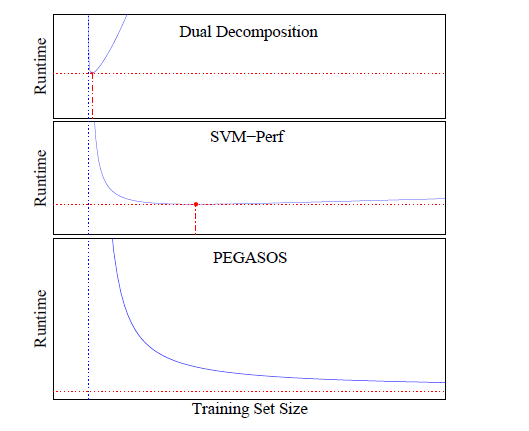
\includegraphics[scale=1]{three_alg.PNG}

%%%%%%%%%%%%%%%%%%%%%%%%%%%%%%%%%%%%%%%%%%%%%%%%%%%%

\section{PAC Learning}

PAC learning is another instance of a problem where more data can be used to speed up computation.

\subsection{Problem Setup}

The problem is called learning the class of \textit{halfspaces over k-sparse vectors}. The space of k-sparse vectors (in dimension $n$) is

$$C_{n, k} = \{x \in \{-1, 0, 1\}^n | |\{i | x_i \neq 0\}| \leq k\}$$

The hypothesis class of halfspaces of k-sparse vectors is

$$\mathcal{H}_{n, k} = \{h_{w, b} : C_{n, k} \rightarrow \{\pm1\} | h_{w, b}(x) = \textrm{sign}(w \cdot x + b), w \in R^n, b \in R\}$$

In the PAC problem, we are given training vectors in $C_{n, k}$ along with +/- labels. The goal is to find the best hypothesis from $\mathcal{H}_{n, k}$.\\

A learning algorithm $L$ maps samples to hypothesis. In the context of this paper the learning algorithm $L$, maps training sets/samples as follows:

$$L : (C_{n,3} \times \{ \pm 1 \} )^m \mapsto \mathcal{H}_{n,3}$$

Notice that the output $L(S)$ of the learning algorithm is a hypothesis $\mathcal{H}_{n,3}$, i.e:

$$L(S) \in \mathcal{H}_{n,3}$$

The error of a hypothesis $h$ w.r.t. $D$, and the error of the class $\mathcal{H}$ w.r.t. $D$ is

$$ Err_{D}(h) = Pr_{(x,y) \sim D} (h(x) \neq y)$$
$$ Err_D(\mathcal{H}) = \min_{h \in \mathcal{H}} Err_D(h)$$

We say $L$ learns $\mathcal{H}_{n,3}$ if for every distribution $D$ on $C_{n,3} \times \{ \pm 1 \}$ and samples $S$ of more than $m(n, \epsilon)$ i.i.d. examples from from $D$:

$$ Pr_{S}[ Err_D(L(S) > Err_D(\mathcal{H}_{n,3}) + \epsilon ] < \frac{1}{10}$$

We say that the learning algorithm is efficient if $L$ returns a hypothesis in $poly(m(n, \epsilon) )$ and the hypothesis can be evaluated in polynomial time.\\

In fact, we could consider a more general problem that allows \textit{improper learning}, where the learning algorithm does not have to choose a hypothesis in $H_{n, k}$, but instead can output one whose error is not much larger than that of the optimal hypothesis in $H_{n, k}$. All of the following results hold for this generalized problem as well, although we will discuss only the original problem.

\subsection{Main Results}

Daniely, Linial, and Shalev-Shwartz give three key results that demonstrate the claim that more data can reduce runtime in this problem of learning the class of $H_{n, 3}$.

\begin{enumerate}

\item It is possible to learn $H_{n, 3}$ using $O(\frac{n}{\epsilon^2})$ training examples.
\item It is possible to learn efficiently (polytime) $H_{n, 3}$ using $\Omega(\frac{n^2}{\epsilon^2})$ training examples.
\item Under a particular assumption regarding the hardness of refuting random 3CNF formulas, it is impossible to learn efficiently $H_{n, 3}$ using $\Omega(\frac{n^{1 + \alpha}}{\epsilon^2})$ training examples, for $\alpha \in [0, .5)$.

\end{enumerate}

The tradeoff between the number of training samples and learning runtime is illustrated below.

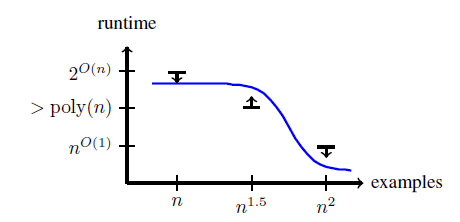
\includegraphics[scale=1]{tradeoff_graph}

Result 1 is easy to show, because $H_{n, 3}$ has VC dimension $n + 1$.
Result 2 is given in Hazan et al. [2012]
We show a slightly stronger version of result 3 in the next section. In particular, define the subclass $H_{n, 3}^d \subset H_{n, 3}$, halfspaces with binary weights, as $H_{n, 3}^d = \{h_{w, 0} | w \in \{\pm 1\}^n\}$. We show that we cannot efficiently learn this subproblem using only $O(\frac{n^{1 + \alpha}}{\epsilon^2})$ examples.

\subsection{Main Theorem}

\textbf{Definitions}

A n-variable 3CNF clause is a boolean formula of the form:

$$C(x) = (-1)^{j_1}x_{i_1} \vee (-1)^{j_2}x_{i_2} \vee (-1)^{j_3}x_{i_3} $$

A 3CNF formula is a boolean formula of the form:

$$ \phi(x) = \wedge^m_{i=1} C_{i}(x) $$

To denote this we use $3CNF_{n,m}$ when it has n variables and m clauses.

Let $Val(\phi)$ denote the maximal fraction of clauses that can be simultaneously satisfied.

If $Val(\phi) =  1$ then we say that $\phi$ is satisfiable.

Boolean formulas can be trivially transformed to formulas with $\{ \pm \}$ instead of $\{ 0,1 \}$ and majority operations.
First the the majority function defined as follows:

$$\forall (x_1, x_2, x_3) \in \{ \pm 1 \}^3, MAJ(x_1, x_2, x_3 ) := sign(x_1 + x_2 + x_3 )$$

An n-variable 3CNF clauses C can be mapped to 3 majority (3MAJ) clauses using the formula:

$$ C(x) = MAJ( (-1)^{j_1}x_{i_1} , (-1)^{j_2}x_{i_2} , (-1)^{j_3}x_{i_3} )$$

An n-variable 3CNF formulas $\phi$ can be equivalently be expressed using 3MAJ formulas as follow:

$$ \phi(x) = \wedge^m_{i=1} C_{i}(x)  = \Pi^m_{i=1} C_{i}(x) $$

To denote this we use $3MAJ_{n,m}$ when it has n variables and m clauses.

\textbf{Conjecture 2.2}: ($\mu$-R3SAT hardness assumption) $\forall \epsilon > 0, \forall \Delta > \Delta_o(\epsilon) $, there exists no efficient algorithm that $\epsilon$-refutes random 3CNF with ratio $\Delta \cdot n^{\mu}$.

%%%% Theorem
\textbf{Theorem 3.1 }: Let $0 \leq \mu \leq 0.5$. If the $\mu$-R3SAT hardness assumption (conjecture 2.2) is true, then there exists no efficient learning algorithm that learns the class $\mathcal{H}_{n,3}$ using $O \left(  \frac{n^{1 + \mu }}{\epsilon^2} \right)$ examples.

To prove theorem 3.1 we will prove a stronger version of it. For that we will need to define:
$$ \mathcal{H}^d_{n,m} = \{ h_{w,0} : C_{n, 3} \mapsto \{ \pm 1\} \mid h_{w,0}(x) = \langle w, x \rangle, w \in R^n, b = 0 \}$$

Notice $\mathcal{H}^d_{n,m} \subset \mathcal{H}_{n,m}$, this fact is what makes theorem 3.2 stronger (and hence imply theorem 3.1):

\textbf{Theorem 3.2 }: Under $\mu$-R3SAT hardness assumption, it is impossible to efficiently learn this subclass  $\mathcal{H}^d_{n,m}$ , using only $O \left(  \frac{n^{1 + \mu }}{\epsilon^2} \right)$.

%%%% PROOF SKETCH
Proof Sketch:

To show that its impossible to learn $\mathcal{H}^d_{n,m}$ (using only $O \left(  \frac{n^{1 + \mu }}{\epsilon^2} \right)$), we will reduce the problem of $\epsilon$-refuting $3MAJ$ formulas to the problem of learning $\mathcal{H}^d_{n,m}$ with $O \left(  \frac{n^{1 + \mu }}{\epsilon^2} \right)$. With this reduction, we will be able to show that if such a learning algorithm $L$ existed, then we could learn $\mathcal{H}^d_{n,m}$ and hence, construct an algorithm that is able to $\epsilon$-refute $3MAJ$ formulas efficiently.

For this reduction to work we will need the following steps:

\textbf{step1)} For this reduction, we will map every 3MAJ clause to two examples in $C_{n,3} \times \{ \pm 1 \}$. Since 3MAJ are just linear combinations of boolen values, we will just indicate the coefficients in the $x_k \in C_{n,3}$ vector. More precisely, for every clause 3MAJ clause $ C(x) = MAJ( (-1)^{j_1}x_{i_1} , (-1)^{j_2}x_{i_2} , (-1)^{j_3}x_{i_3} )$ one can map it to an example $(x_k , y_k) \in C_{n , 3} \times \{ \pm 1\}$ by choosing $b \in \{ \pm 1\}$ (at random) and letting:

$$(x_k, y_k) = b (\sum^3_{l=1} (-1)^{j_l} e_{i_l}, 1) \in (C_{n,3} \times \{ \pm 1 \})$$

where $e_i$ are the usual standard basis vectors.
Conceptually, we are simply using the indices of the boolean vector take part of the current 3MAJ formula to denote the non-zero relevant entries in the vector $x_k$.
The vector $y_k$ is intended to indicate if the current clause is satisfied or not.

\textbf{step2)} Apart from mapping each clause $C(x)$ we will also map every possible $w \in\mathcal{H}^d_{n,m}$ to a possible (boolean) assignment $\psi $ to the 3MAJ formula $\phi(x)$.
To do this we will take advantage that $w \in \{ \pm 1 \}^n $ and that there is a bijection with vectors $w \in \{ \pm 1 \}^n $ to hyperplanes in $\mathcal{H}^d_{n,m}$.

For this proof to work the following fact is crucial:

\textbf{step3} Claim: If $\psi \in \{ \pm 1 \}^n $ and its corresponding hypothesis are $h_{\psi, 0} (x) = sign ( \langle \psi , x \rangle )$, then $h_{\psi, 0} (x_k) = y_k$ if and only if $\psi$ satisfies $C_k$.

Sketch proof:

This fact is nearly immediate because we constructed $x_k$ to be the "coefficients" of the majority formula but without the actual boolean values $x$. Therefore one can appreciate that the inner product  $ \langle \psi , x \rangle $ simply linearly combines the coefficients of 3MAJ (encoded in $x_k$) and with the satisfying assigning $\psi \in \{ \pm 1\}^n$. Since $y_k$ is always flipped depending whether $b$ is 1 or -1, $y_k$ matches $\langle \psi , x \rangle $ if and only if $C(x)$ is satisfied.

\textbf{step4} Given $\phi \in 3MAJ_{n, \Delta n^{1 + \mu}}$ (and for large enough $\Delta$) consisting of 3MAJ clauses $C_1, ..., C_{\Delta n^{1 + \mu}}$ we will create a sample set S consisting of $\Delta n^{1 + \mu}$ examples $(x_k, y_k)$ for each clause $C_k$ as described in step 2. Now given these samples we will choose a random subset $S_1$ of size $O(\frac{n^{1+\mu}}{\epsilon} )$. Let the empirical distribution induced by choosing $(C_{n,3} \times \{ \pm 1\})$ from $\phi$ be $D$. Let the learned hypothesis be denoted by $L(S)$.

Now with these ingredients we can use the learned hypothesis $L(S)$ to, to see what fraction of clauses are actually satisfiable or not (i.e. which are random). This is equivalent to constructing an algorithm A that reliable refutes $\phi$ formulas.

If $\phi$ is nearly satisfiable, i.e. $Val(\phi) \geq 1 - \epsilon$, then, most of the clauses that were mapped to $(x_k, y_k)$ will have a vector $x_k$ that is satisfiable and hence, matches $y_k$. If this is the case then $L(S)$ will get most of its predictions correct (with high probability, since our learning algorithm is PAC learnable and only learns successfully with high probability). Therefore $ Err_{D}(L(S)) $ will be small w.h.p. If this is the case our algorithm will return "exceptional" (and its likely to be satisfiable).

On the other hand, if $\phi$ is random, then no algorithm can learn $\phi$. Why? Well, if $\phi$ is random then for every $(x_k, y_k)$, $y_k$ will be a Bernoulli r.v. with parameter $\frac{1}{2}$, independent of $x_k$. Since the instances is basically random and the algorithm was only provided with $O(\frac{n^{1+\mu}}{\epsilon} )$, the learning algorithm will not see most of the clauses and therefore, since its seeing something that is random by change, will produce a hypothesis that is independent of its observations. Since these clauses are random, h is likely to make a mistake on about half of the clauses. Therefore, $Err_{D}(L(S))$ will be close to 1/2 (considered "large", i.e. it makes a large mistake). Therefore, output "typical".

Therefore, in summary, if $Err_{D}(L(S))$ is large output "typical", otherwise, if the error $Err_{D}(L(S))$ is small output "exceptional".

Therefore, we have constructed an efficient algorithm with small sample complexity that $\epsilon$-refutes 3MAJ formulas, which should not be possible under conjecture 2.2.

\subsection{Open Questions}

It is unknown how efficiently we can learn the problem using $O(\frac{n^{1 + \beta}}{\epsilon^2})$ examples, where $\beta \in [.5, 1)$. Daniely et al conjecture that the problem can be learned in polynomial time using $O(\frac{n^{1.5}}{\epsilon^2})$ examples.

\end{document} 